\documentclass{article}
%DIF LATEXDIFF DIFFERENCE FILE
%DIF DEL main_accepted.tex   Wed Oct 14 12:27:50 2026
%DIF ADD main.tex            Wed Oct 14 15:33:16 2026
\usepackage{stywhispers}
%DIF 3a3-7
\makeatletter % captions in 9 pt (\small of the 10 pt body) %DIF > 
\long\def\@makecaption#1#2{\vskip 6pt %DIF > 
 \setbox\@tempboxa\hbox{\small #1. #2} %DIF > 
 \ifdim\wd\@tempboxa>\hsize {\small #1. #2\par}\else\hbox to\hsize{\hfil\box\@tempboxa\hfil}\fi} %DIF > 
\makeatother %DIF > 
%DIF -------
\usepackage{cite}
\usepackage{amsmath,amssymb,amsfonts}
\usepackage{mathtools}
\usepackage{graphicx}
\usepackage{booktabs}
\usepackage{array}
\usepackage{textcomp}
\usepackage{url}
\usepackage{dblfloatfix}

\graphicspath{{figures/}}
\makeatletter %DIF > 
\raggedbottom %DIF > 
\setlength{\parskip}{0pt} %DIF > 
\setlength{\textfloatsep}{9pt}\setlength{\floatsep}{8pt}\setlength{\intextsep}{8pt} %DIF > 
\setcounter{dbltopnumber}{3}\renewcommand{\dbltopfraction}{0.95}\renewcommand{\dblfloatpagefraction}{0.6} %DIF > 
\setlength{\dbltextfloatsep}{9pt}\setlength{\dblfloatsep}{8pt} %DIF > 
\setlength{\abovecaptionskip}{0pt}\setlength{\belowcaptionskip}{0pt} %DIF > 
\renewcommand\section{\@startsection{section}{1}{\z@}{9pt}{4pt}{\normalfont\bfseries}} %DIF > 
\renewcommand\subsection{\@startsection{subsection}{2}{\z@}{7pt}{3pt}{\normalfont\bfseries}} %DIF > 
\renewcommand\subsubsection{\@startsection{subsubsection}{3}{\z@}{6pt}{2pt}{\normalfont\itshape}} %DIF > 
\makeatother %DIF > 
%DIF PREAMBLE EXTENSION ADDED BY LATEXDIFF
\RequirePackage[normalem]{ulem} %DIF PREAMBLE
\RequirePackage{color} %DIF PREAMBLE
\providecommand{\DIFadd}[1]{{\protect\color[rgb]{0.85,0,0}#1}} %DIF PREAMBLE
\providecommand{\DIFdel}[1]{{\protect\color[gray]{0.5}\sout{#1}}} %DIF PREAMBLE
\providecommand{\DIFaddbegin}{} %DIF PREAMBLE
\providecommand{\DIFaddend}{} %DIF PREAMBLE
\providecommand{\DIFdelbegin}{} %DIF PREAMBLE
\providecommand{\DIFdelend}{} %DIF PREAMBLE
\providecommand{\DIFmodbegin}{} %DIF PREAMBLE
\providecommand{\DIFmodend}{} %DIF PREAMBLE
\providecommand{\DIFaddFL}[1]{\DIFadd{#1}} %DIF PREAMBLE
\providecommand{\DIFdelFL}[1]{\DIFdel{#1}} %DIF PREAMBLE
\providecommand{\DIFaddbeginFL}{} %DIF PREAMBLE
\providecommand{\DIFaddendFL}{} %DIF PREAMBLE
\providecommand{\DIFdelbeginFL}{} %DIF PREAMBLE
\providecommand{\DIFdelendFL}{} %DIF PREAMBLE
%DIF AMSMATHULEM PREAMBLE %DIF PREAMBLE
\makeatletter %DIF PREAMBLE
\let\sout@orig\sout %DIF PREAMBLE
\renewcommand{\sout}[1]{\ifmmode\text{\sout@orig{\ensuremath{#1}}}\else\sout@orig{#1}\fi} %DIF PREAMBLE
\makeatother %DIF PREAMBLE
%DIF COLORLISTINGS PREAMBLE %DIF PREAMBLE
\RequirePackage{listings} %DIF PREAMBLE
\RequirePackage{color} %DIF PREAMBLE
\lstdefinelanguage{DIFcode}{ %DIF PREAMBLE
%DIF DIFCODE_UNDERLINE %DIF PREAMBLE
  moredelim=[il][\color{red}\sout]{\%DIF\ <\ }, %DIF PREAMBLE
  moredelim=[il][\color{blue}\uwave]{\%DIF\ >\ } %DIF PREAMBLE
} %DIF PREAMBLE
\lstdefinestyle{DIFverbatimstyle}{ %DIF PREAMBLE
	language=DIFcode, %DIF PREAMBLE
	basicstyle=\ttfamily, %DIF PREAMBLE
	columns=fullflexible, %DIF PREAMBLE
	keepspaces=true %DIF PREAMBLE
} %DIF PREAMBLE
\lstnewenvironment{DIFverbatim}[1][]{\lstset{style=DIFverbatimstyle}}{} %DIF PREAMBLE
\lstnewenvironment{DIFverbatim*}[1][]{\lstset{style=DIFverbatimstyle,showspaces=true}}{} %DIF PREAMBLE
\lstset{extendedchars=\true,inputencoding=utf8}

%DIF END PREAMBLE EXTENSION ADDED BY LATEXDIFF

\begin{document}
\ninept

\title{SpectralForge: A Physics-Based Simulator for Fluorescence Hyperspectral Imaging}

\name{Narek Meloyan$^{1,2,3}$, Narine Sarvazyan$^{1,3,4}$}
\address{$^{1}$Akian College of Science and Engineering, American University of Armenia, Yerevan, Armenia \\
$^{2}$Engineering Research Center, American University of Armenia, Yerevan, Armenia \\
$^{3}$L.A.\ Orbeli Institute of Physiology NAS RA, Yerevan, Armenia \\
$^{4}$George Washington University, Washington, DC, USA \\
\texttt{narek.h.meloyan@gmail.com}, \texttt{phynas@gwu.edu}}

\maketitle

\begin{abstract}
\noindent\fbox{\parbox{0.94\columnwidth}{\scriptsize\textbf{Changes vs.\ accepted version: additions in \textcolor[rgb]{0.85,0,0}{red}, deletions \textcolor[gray]{0.5}{\sout{struck through in grey}}.} (Review copy; this file may exceed five pages. The submission file is \texttt{main.pdf}, 5 pages.) Summary: a new Sec.~2.6 and Fig.~6 compare the Eq.~(1) model with real measurements: a drop at held-out excitations, and real collagen measured vs.\ predicted spectra at held-out excitations with a residual strip, with held-out error over 24 collagen cases (SAM $8.4\pm1.8^\circ$, shape $R^2=0.83\pm0.13$, relative RMS $0.097\pm0.023$; the empirical copy is slightly better, emission shape only). Also added: a two-level validity paragraph at the start of Sec.~3, a setup summary table (Table~1), a spectral-grid subsection (564 bands explained), the Studio workbench figure, and one abstract clause; Eq.~(2) corrected (inner filter and reabsorption), several numbers replaced by values from the correct runs, previously uncited references cited, and the Evaluation, Benchmark and Discussion text tightened to stay at five pages (limitations content kept). Layout: figures enlarged (Figs.~1--6), captions in 9~pt. Acknowledgment: the United States R44 HL120511 award was removed.}}\par\medskip


Acquiring four-dimensional fluorescence hyperspectral data is slow and costly. An
instrument records a full emission spectrum at each of several excitation wavelengths and
for every pixel, fluorescence signals are weak and easily buried in scatter and
autofluorescence, and the illumination needed to raise them photobleaches the sample, so a
single cube can consume hours of scarce instrument time. This makes it hard to plan
acquisitions, prototype processing methods, or build shared benchmarks. We present
\textbf{SpectralForge}, an open, physics-based simulator that renders realistic 4D
excitation-emission cubes with perfect ground truth from a parametric fluorophore model
obeying the standard laws of fluorescence photophysics (Kasha, Vavilov, Franck-Condon,
Stokes shift), with optional inner-filter attenuation, reabsorption, Foerster resonance
energy transfer (FRET), scatter, photon and read noise, and instrument clutter. Because
every rendered cube comes with its concentration maps and true emission peaks, a method can
be developed, tested, and compared before any measurement is taken. As \DIFdelbegin \DIFdel{one }\DIFdelend \DIFaddbegin \DIFadd{a }\DIFaddend worked
example, we \DIFdelbegin \DIFdel{use the simulator to }\DIFdelend study spectral band selection, where the goal is to keep
only the informative bands and so acquire or process less. Scenes are built so that band
variance is decoupled from class informativeness (measured correlation $\approx -0.1$), so the
task is not solved by variance ranking, and two controls, a random baseline and the full
spectrum, tell a real gain from a chance one. \DIFdelbegin \DIFdel{Running }\DIFdelend \DIFaddbegin \DIFadd{Fitting the model to measured drop and collagen spectra tests it against real data, and running }\DIFaddend a panel of selectors through the
simulator shows it behaving as designed and marks where label-free selection helps and
where it does not. SpectralForge and its workbench are in active development, with early
access \DIFdelbegin \DIFdel{available to }\DIFdelend \DIFaddbegin \DIFadd{for }\DIFaddend interested labs on request; the full study is released for reproducible
use in 4D fluorescence imaging.
\end{abstract}

\begin{keywords}
fluorescence hyperspectral imaging, physics-based simulation, synthetic data,
excitation-emission, photophysics, band selection.
\end{keywords}

\section{Introduction}
A multi-excitation fluorescence measurement illuminates a sample at several excitation
wavelengths and, for each, records an emission spectrum\DIFdelbegin \DIFdel{across many bands}\DIFdelend . Every pixel therefore carries an
excitation-emission matrix (EEM), and an image is a four-dimensional array over excitation,
emission, height, and width (Fig.~\ref{fig:cube4d}). \DIFdelbegin \DIFdel{The modality is useful because
different fluorophores}\DIFdelend \DIFaddbegin \DIFadd{Fluorophores}\DIFaddend , tissue states, \DIFdelbegin \DIFdel{or }\DIFdelend \DIFaddbegin \DIFadd{and }\DIFaddend species
separate in this joint \DIFdelbegin \DIFdel{excitation-emission }\DIFdelend domain, which is why it is used \DIFdelbegin \DIFdel{across }\DIFdelend \DIFaddbegin \DIFadd{for }\DIFaddend biomedical and material imaging,
for example label-free imaging of cardiac tissue by its endogenous
autofluorescence~\cite{ref_mercader,ref_gil}. \DIFdelbegin \DIFdel{Adding excitation wavelengths turns each
single spectrum into an excitation-emission matrix that separates overlapping
fluorophores }\DIFdelend \DIFaddbegin \DIFadd{Added excitations separate overlapping
fluorophores that }\DIFaddend a single-excitation \DIFdelbegin \DIFdel{hyperspectral }\DIFdelend image cannot, \DIFdelbegin \DIFdel{which improves downstream }\DIFdelend \DIFaddbegin \DIFadd{improving }\DIFaddend tissue and material
classification~\cite{ref_chil4d,ref_chillichen,ref_hunanyan}\DIFdelbegin \DIFdel{.
It is also expensive to acquire. Each added excitation }\DIFdelend \DIFaddbegin \DIFadd{, but each one }\DIFaddend multiplies the
acquisition by a full emission scan, \DIFdelbegin \DIFdel{fluorescence }\DIFdelend signals are weak \DIFdelbegin \DIFdel{and easily lost in }\DIFdelend \DIFaddbegin \DIFadd{against }\DIFaddend scatter and autofluorescence,
and \DIFdelbegin \DIFdel{the illumination needed to raise them photobleaches the very
molecules being measured}\DIFdelend \DIFaddbegin \DIFadd{illumination photobleaches the sample}\DIFaddend . A single \DIFdelbegin \DIFdel{high-quality }\DIFdelend 4D cube can \DIFdelbegin \DIFdel{therefore }\DIFdelend consume hours of
\DIFdelbegin \DIFdel{specialized instrument time , }\DIFdelend \DIFaddbegin \DIFadd{instrument time }\DIFaddend and labeled real cubes remain scarce.

\DIFdelbegin \DIFdel{This scarcity slows everything downstream. }\DIFdelend Planning an acquisition, prototyping a processing method, or comparing algorithms all
ideally happen before instrument time is committed, yet each needs representative data, and
real cubes carry no ground truth \DIFdelbegin \DIFdel{: there
is no reference for }\DIFdelend \DIFaddbegin \DIFadd{about }\DIFaddend which fluorophores are where or which bands \DIFdelbegin \DIFdel{truly }\DIFdelend matter. A
physically realistic simulator \DIFdelbegin \DIFdel{addresses both problems at once. If it }\DIFdelend \DIFaddbegin \DIFadd{that }\DIFaddend renders cubes from the \DIFdelbegin \DIFdel{actual
}\DIFdelend laws of fluorescence and returns
the underlying concentrations and emission peaks \DIFdelbegin \DIFdel{, }\DIFdelend \DIFaddbegin \DIFadd{addresses both problems: }\DIFaddend a method can be
built, tested, and benchmarked against an answer key, and only the promising design need
\DIFdelbegin \DIFdel{ever }\DIFdelend reach the instrument.

This paper presents \textbf{SpectralForge}, an open simulator of that kind for 4D
fluorescence imaging, with an interactive workbench for building scenes by hand and a small
library for scripting them. To show the tool at work we take one concrete task, spectral
band selection, and run a study through it end to end: the simulator provides the cubes and
their ground truth, a controlled evaluation protocol scores the candidate selectors, and
the results show both that the tool behaves as designed and where a learned selector
actually helps. Band selection is only one use\DIFdelbegin \DIFdel{. The }\DIFdelend \DIFaddbegin \DIFadd{; the }\DIFaddend same generator supports experiment
planning, \DIFdelbegin \DIFdel{algorithm prototyping, teaching, and any study that benefits from 4D fluorescence
data with a known answer}\DIFdelend \DIFaddbegin \DIFadd{prototyping, and teaching}\DIFaddend .

\begin{figure*}[!tb]
\centering
\DIFdelbeginFL %DIFDELCMD < 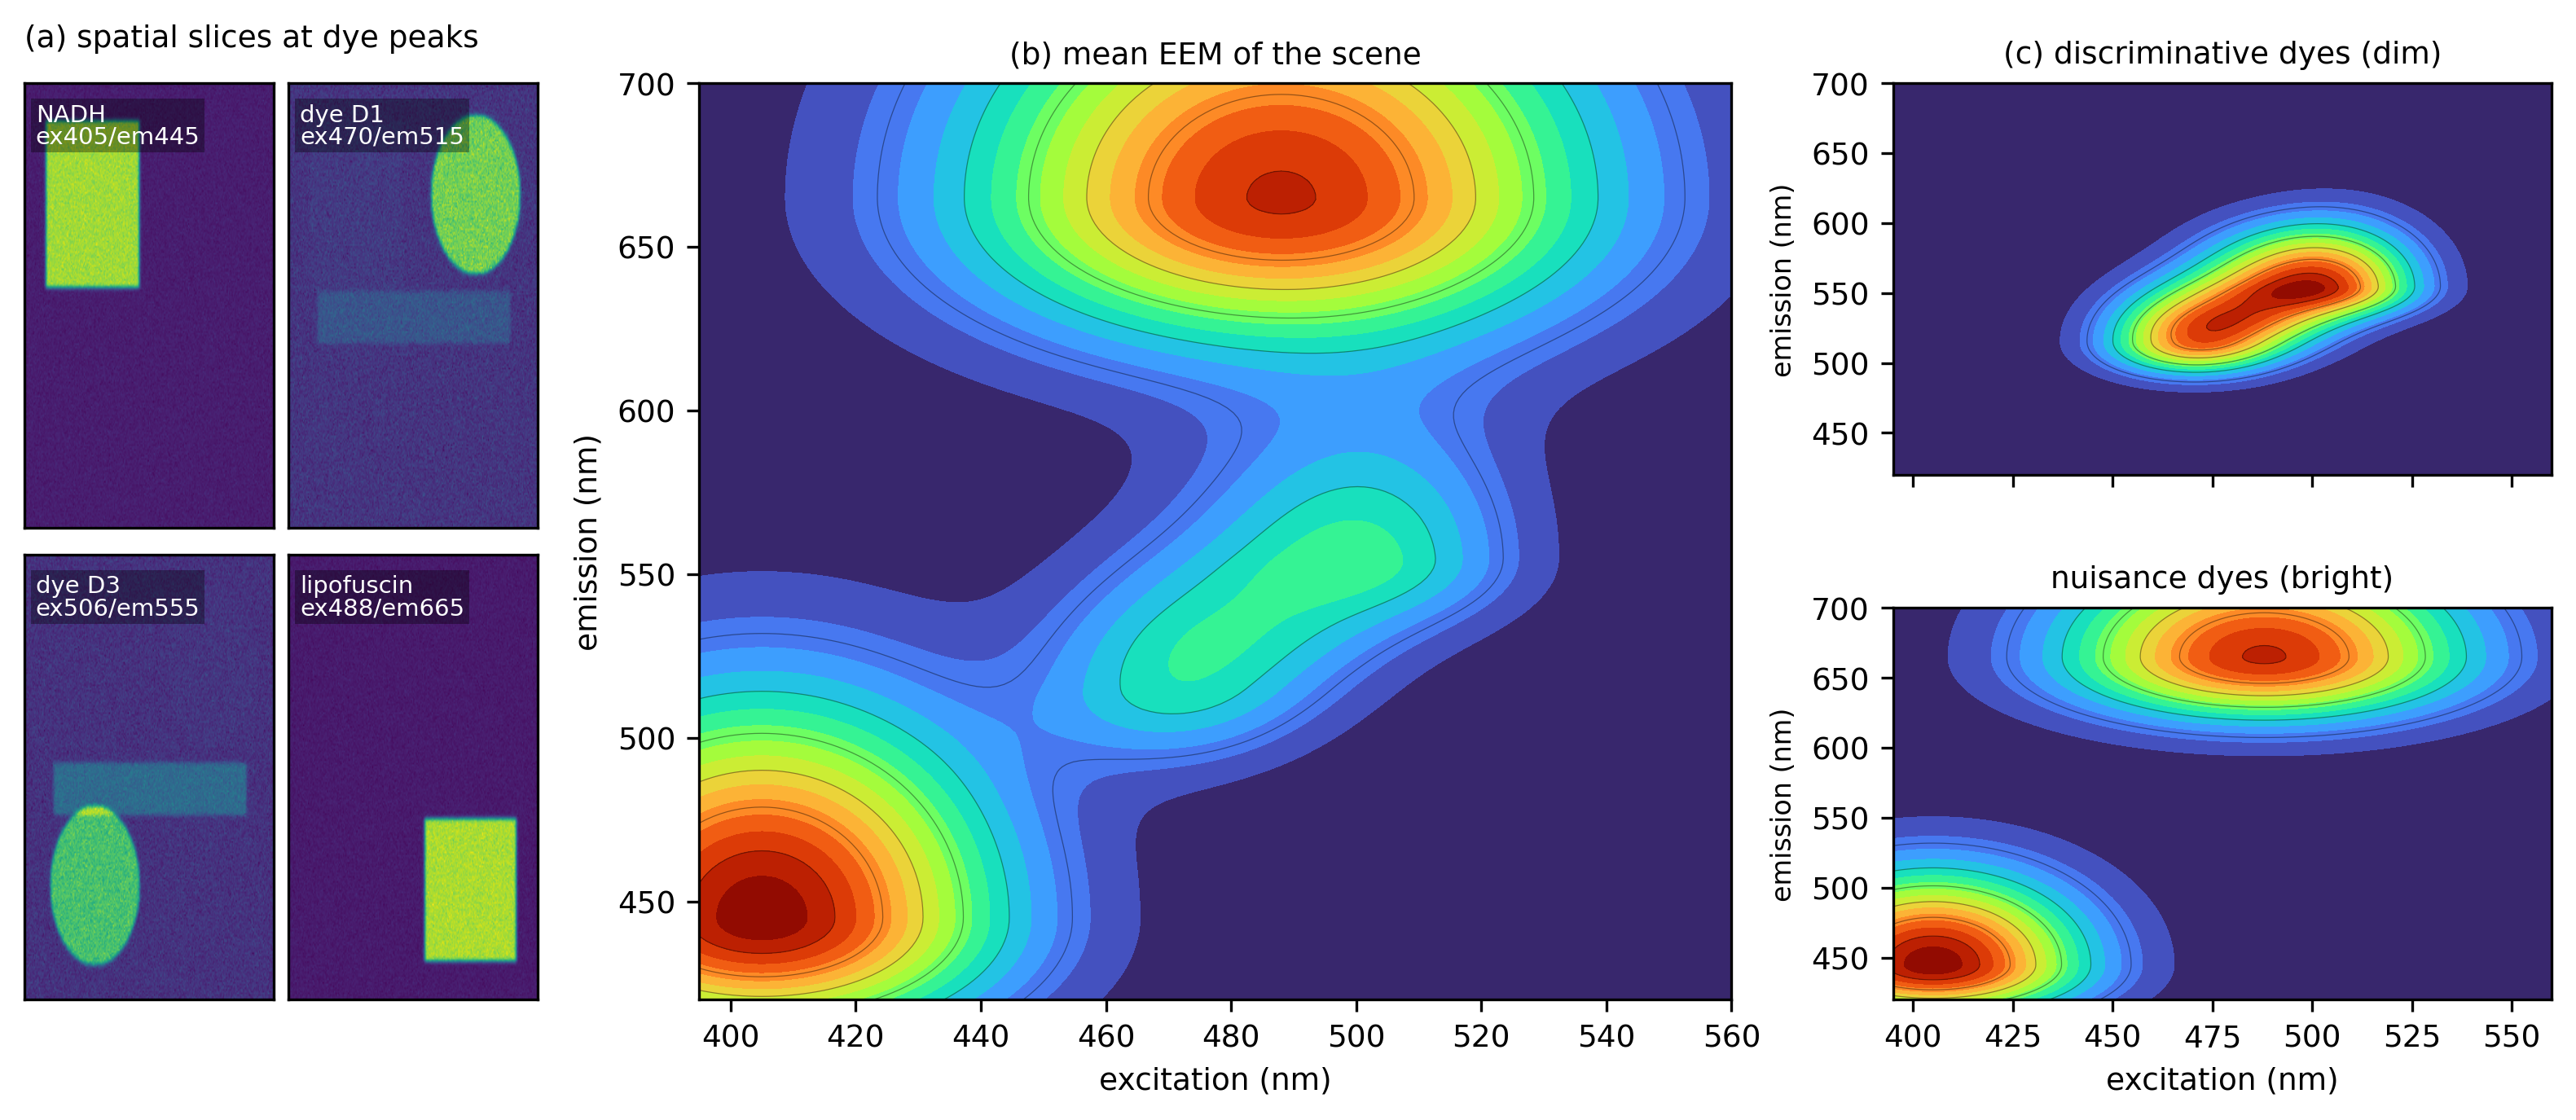
\includegraphics[width=0.99\textwidth]{fig_cube4d.png}
%DIFDELCMD < %%%
\DIFdelendFL \DIFaddbeginFL 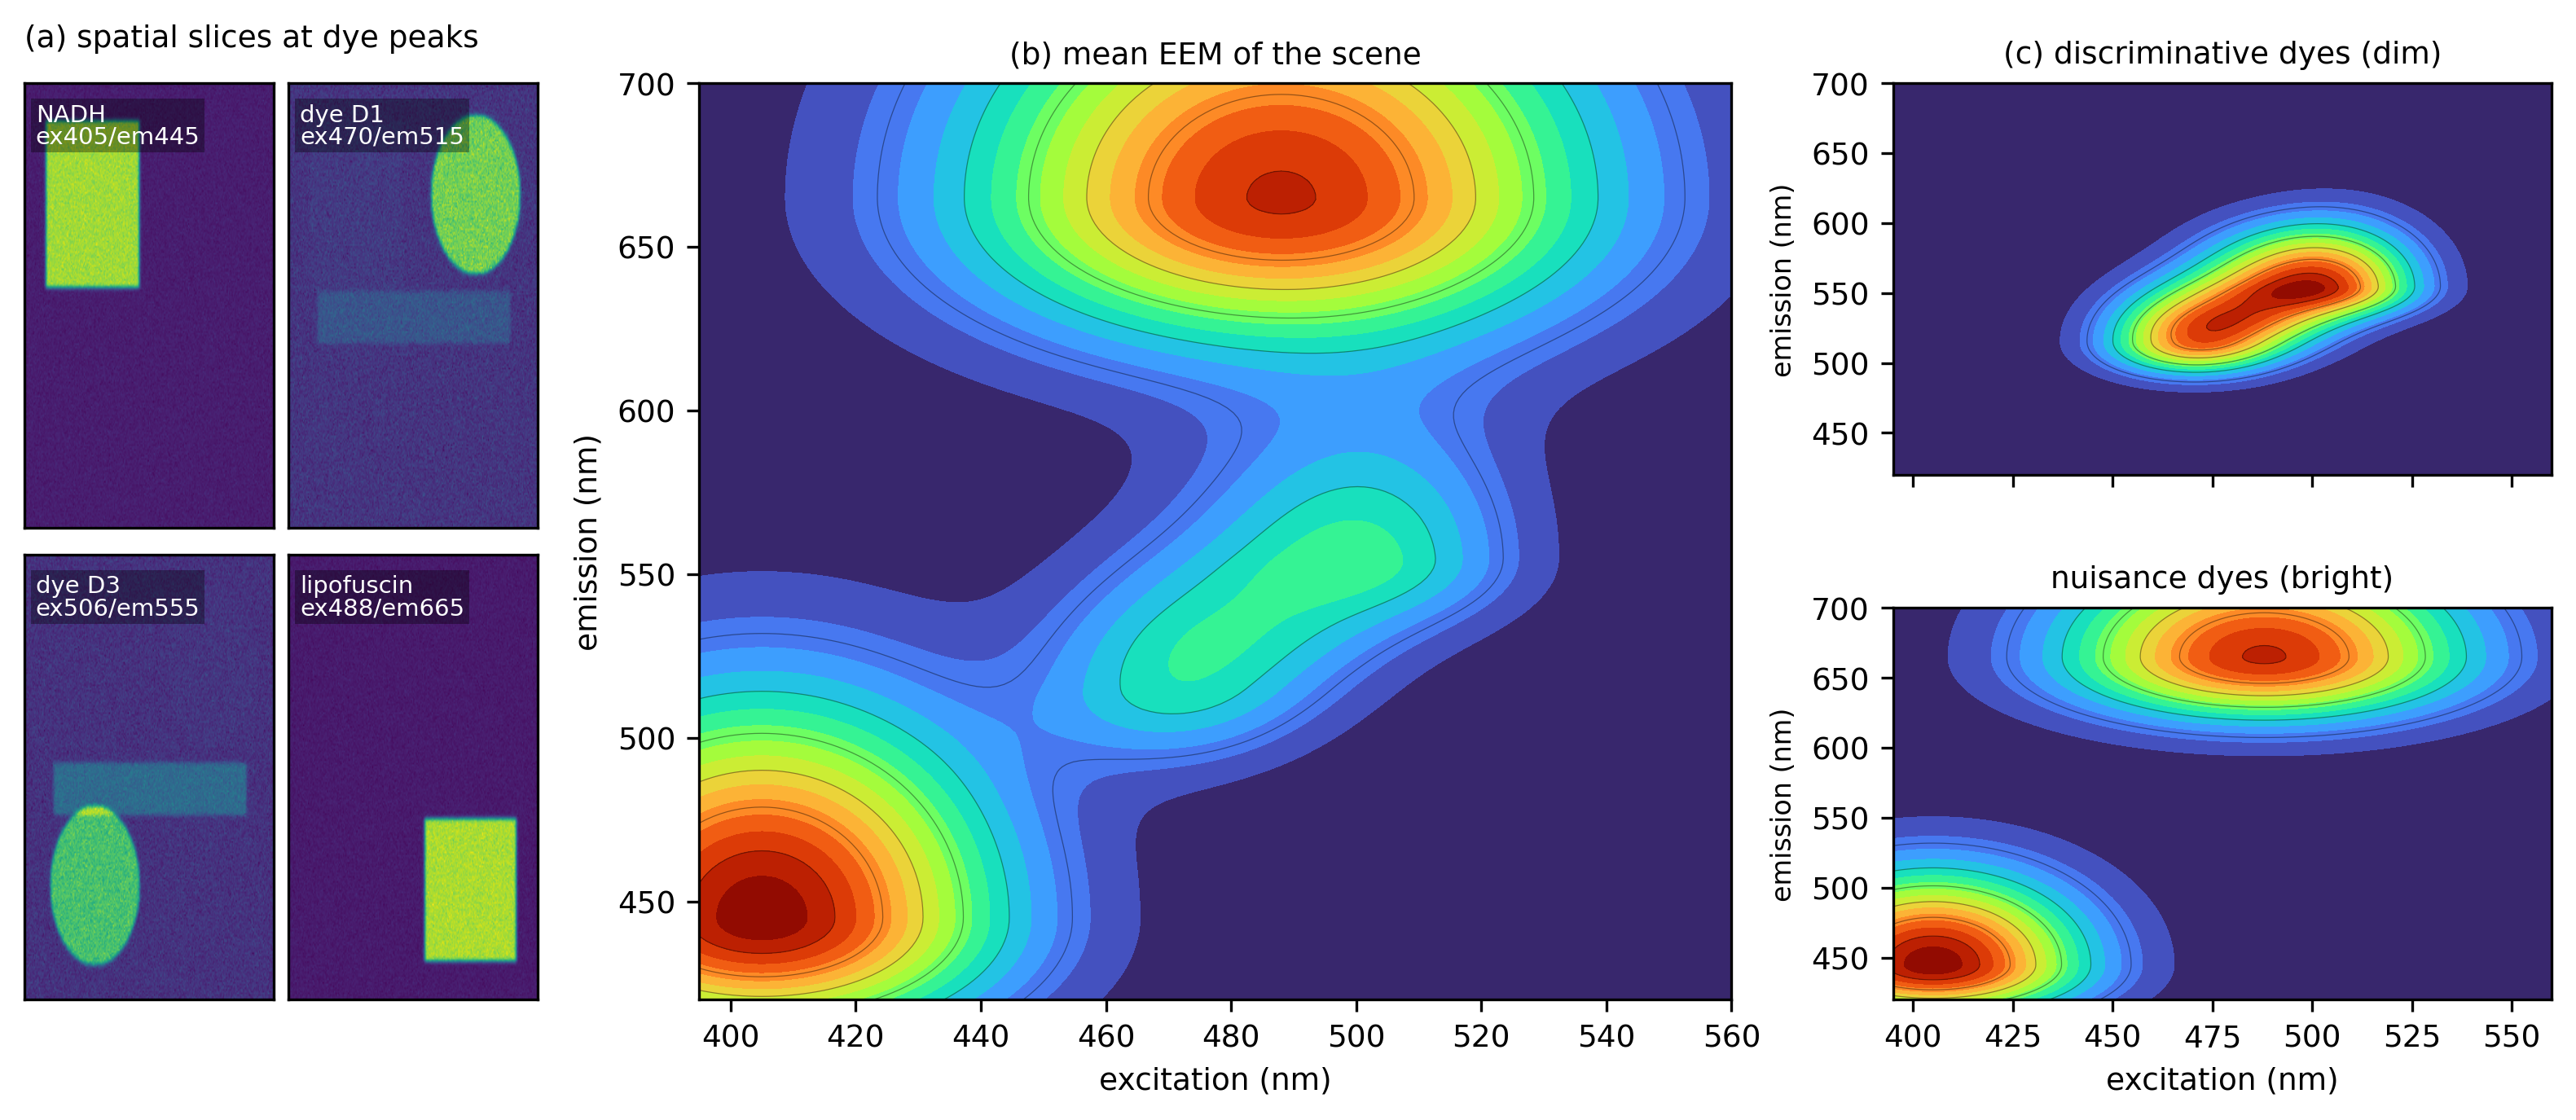
\includegraphics[width=0.96\textwidth]{fig_cube4d.png}
\DIFaddendFL \caption{A rendered 4D fluorescence cube from SpectralForge, \DIFdelbeginFL \DIFdelFL{here }\DIFdelendFL an example scene \DIFdelbeginFL \DIFdelFL{painted
in the workbench }\DIFdelendFL with each dye laid
down as a shape. (a) \DIFdelbeginFL \DIFdelFL{A slice of the cube taken }\DIFdelendFL \DIFaddbeginFL \DIFaddFL{Slices }\DIFaddendFL at each dye's emission peak \DIFdelbeginFL \DIFdelFL{reveals that dye's }\DIFdelendFL \DIFaddbeginFL \DIFaddFL{reveal its }\DIFaddendFL painted region\DIFdelbeginFL \DIFdelFL{(NADH square, dyes D1/D3 disks,
lipofuscin block)}\DIFdelendFL ; \DIFdelbeginFL \DIFdelFL{a slice lights up only dyes that both absorb at its excitation and emit
at its emission, so }\DIFdelendFL every pixel
effectively stores an \DIFdelbeginFL \DIFdelFL{excitation-emission matrix (}\DIFdelendFL EEM\DIFdelbeginFL \DIFdelFL{)}\DIFdelendFL . (b) The mean EEM\DIFdelbeginFL \DIFdelFL{of the scene is the familiar fluorescence landscape}\DIFdelendFL : each fluorophore is a smooth blob at its excitation
and (Stokes-shifted) emission. (c) \DIFdelbeginFL \DIFdelFL{Decomposed by }\DIFdelendFL \DIFaddbeginFL \DIFaddFL{By }\DIFaddendFL role, the discriminative dyes form \DIFdelbeginFL \DIFdelFL{a single }\DIFdelendFL \DIFaddbeginFL \DIFaddFL{one }\DIFaddendFL dim, overlapping
cluster while the class-irrelevant nuisance dyes are bright and well separated, so band
variance is dominated by \DIFdelbeginFL \DIFdelFL{the
}\DIFdelendFL uninformative signal.}
\label{fig:cube4d}
\end{figure*}

\section{The SpectralForge Forward Model}
\subsection{Photophysics}
The generator is built on the physics of fluorescence\DIFaddbegin \DIFadd{~\mbox{%DIFAUXCMD
\cite{ref_lakowicz,ref_valeur} }\hskip0pt%DIFAUXCMD
}\DIFaddend so that ``informative''
means what it means physically. A fluorophore absorbs a photon, relaxes
non-radiatively to the lowest vibrational level of the first excited singlet, and
emits \DIFaddbegin \DIFadd{(the Jab\l{}o\'nski picture~\mbox{%DIFAUXCMD
\cite{ref_jablonski}}\hskip0pt%DIFAUXCMD
)}\DIFaddend . Four consequences shape the EEM. By \emph{Kasha's rule}\DIFaddbegin \DIFadd{~\mbox{%DIFAUXCMD
\cite{ref_kasha} }\hskip0pt%DIFAUXCMD
}\DIFaddend emission occurs from
that lowest level regardless of the excitation, so the emission shape is independent
of excitation wavelength and the EEM is approximately trilinear (an excitation
profile times an emission profile times a concentration map), the basis of PARAFAC\DIFaddbegin \DIFadd{~\mbox{%DIFAUXCMD
\cite{ref_bro}}\hskip0pt%DIFAUXCMD
}\DIFaddend .
By \emph{Vavilov's rule} the quantum yield is, to first order, independent of
excitation; only the amount absorbed changes. The \emph{Franck-Condon} principle sets
the broadened, roughly mirror-image band envelopes and an optional vibronic shoulder
about $1300\,\mathrm{cm}^{-1}$ to the red. The \emph{Stokes shift} red-shifts emission
relative to absorption. \DIFaddbegin \DIFadd{Together these rules fix the structure of the forward model below; the departures from them that matter in practice (inner-filter attenuation, reabsorption, and FRET) enter as optional, switchable effects (Sec.~\ref{sec:artifacts}).
}\DIFaddend 

\subsection{Trilinear render and the additive invariant}
Each fluorophore $k$ is a parametric model with a peak-normalized Gaussian excitation
profile $a_k(\lambda_\mathrm{ex})$ and an area-normalized emission profile
$e_k(\lambda_\mathrm{em})$, extinction $\varepsilon_k$, quantum yield $\Phi_k$, and a
per-pixel concentration map $c_k(x,y)$. The rendered cube is a dilute linear
superposition,
\begin{equation}
F(x,y,\lambda_\mathrm{ex},\lambda_\mathrm{em}) = g \sum_k
c_k(x,y)\,\varepsilon_k\,\Phi_k\,a_k(\lambda_\mathrm{ex})\,e_k(\lambda_\mathrm{em}),
\end{equation}
where $g$ folds lamp, exposure, and power. \DIFdelbegin \DIFdel{This is Kasha's rule written as algebra.
The profiles are Gaussian , $a_k$ peak-normalized and $e_k$ area-normalized with widths $\mathrm{FWHM}/(2\sqrt{2\ln 2})$, and
a fluorophore's brightness is the product
}\DIFdelend \DIFaddbegin \DIFadd{Gaussian widths are $\sigma=\mathrm{FWHM}/(2\sqrt{2\ln 2})$, and
brightness is }\DIFaddend $\varepsilon_k\Phi_k$.
With all optional physics and artifacts off the model is \emph{exactly linear},
$\mathrm{render}(A{+}B)=\mathrm{render}(A){+}\mathrm{render}(B)$, an invariant the
implementation tests; difficulty is then added in realistic, opt-in
increments. A per-pixel class label is the argmax over the discriminative
fluorophores. Fig.~\ref{fig:fluoro} shows the fluorophore model.

\begin{figure}[t]
\centering
\DIFdelbeginFL %DIFDELCMD < 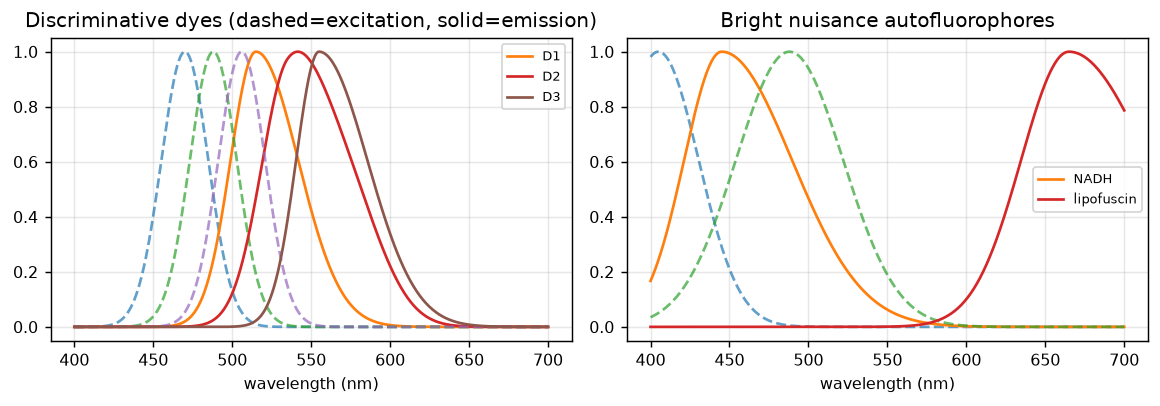
\includegraphics[width=\linewidth]{fig_fluorophores.png}
%DIFDELCMD < %%%
\DIFdelendFL \DIFaddbeginFL 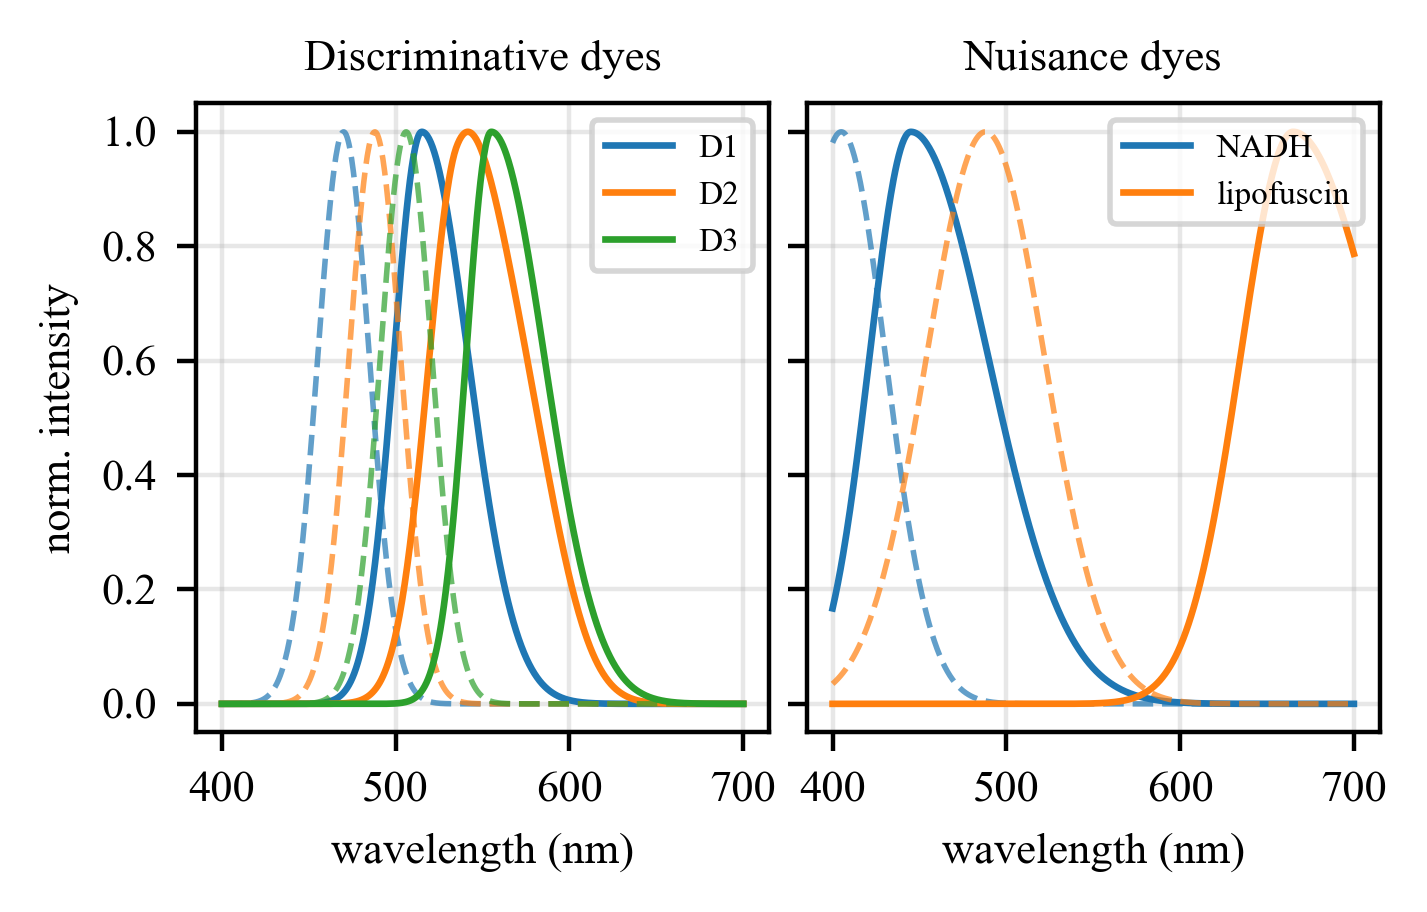
\includegraphics[width=\columnwidth]{fig_fluorophores_v2.png}
\DIFaddendFL \caption{Parametric fluorophore spectra \DIFdelbeginFL \DIFdelFL{. Left: three discriminative dyes }\DIFdelendFL (dashed, excitation; solid, emission)\DIFdelbeginFL \DIFdelFL{of modest brightness with }\DIFdelendFL \DIFaddbeginFL \DIFaddFL{. Left: three dim, }\DIFaddendFL overlapping \DIFdelbeginFL \DIFdelFL{emission and
distinct excitation}\DIFdelendFL \DIFaddbeginFL \DIFaddFL{discriminative dyes}\DIFaddendFL . Right: two bright nuisance autofluorophores that dominate band variance but carry no class information.}
\label{fig:fluoro}
\end{figure}

\subsection{Variance is decoupled from informativeness}
The central design choice is the scene generator. Discriminative dyes are painted with
smooth random concentration fields whose per-pixel argmax defines the class; they are
dim and spectrally overlapping, so their content lives in low-variance band \emph{shape},
while independent nuisance dyes are bright but class-irrelevant (Fig.~\ref{fig:cube4d}c).
\DIFdelbegin \DIFdel{Real photophysics compounds the decoupling: scatter ridgesand bright autofluorescence}\DIFdelend \DIFaddbegin \DIFadd{Scatter ridges, bright autofluorescence, and shot noise }\DIFaddend add high-variance but class-irrelevant
signal\DIFdelbegin \DIFdel{, shot noise inflates bright redundant bands,
and the discriminative signal sits in dim or subtly shaped bands}\DIFdelend . On a confounded scene the correlation between per-band variance and per-band
discriminability is $\approx -0.1$, versus strongly positive on \DIFdelbegin \DIFdel{naive }\DIFdelend clean data, so the
highest-variance bands \DIFdelbegin \DIFdel{carry no class
information }\DIFdelend \DIFaddbegin \DIFadd{are uninformative }\DIFaddend (Fig.~\ref{fig:scene}) and \DIFdelbegin \DIFdel{a variance ranker cannot solve the task}\DIFdelend \DIFaddbegin \DIFadd{variance ranking fails}\DIFaddend .

\begin{figure}[t]
\centering
\DIFdelbeginFL %DIFDELCMD < 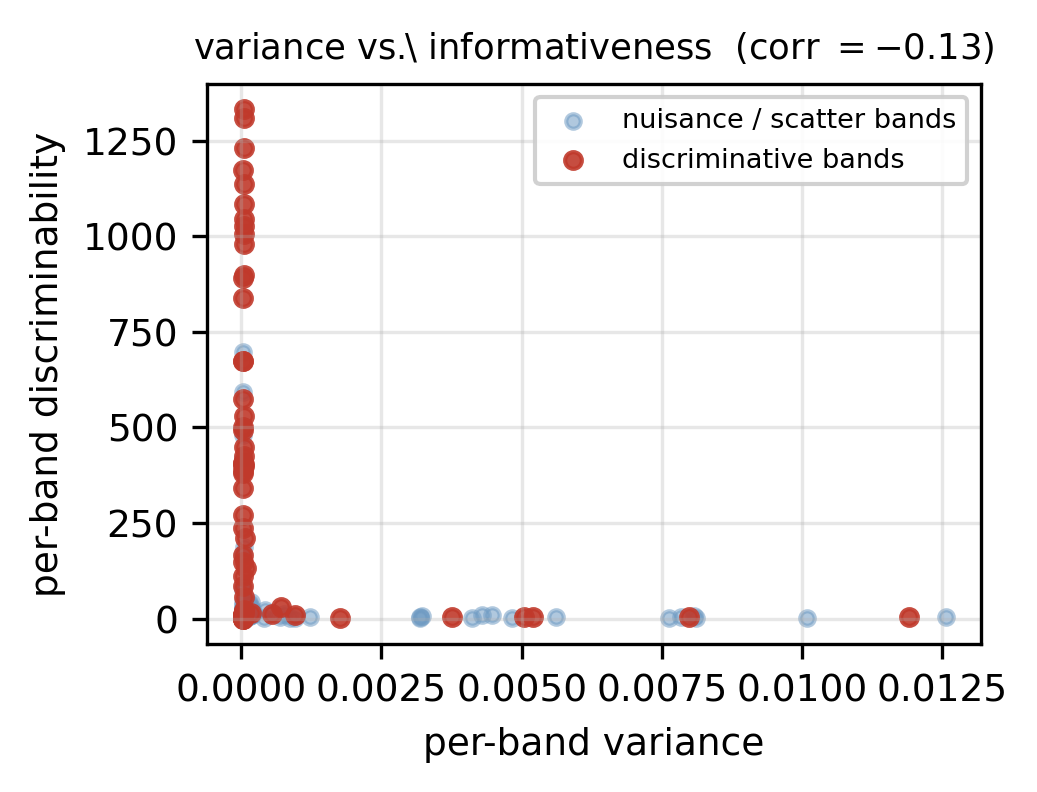
\includegraphics[width=0.94\linewidth]{fig_scene.png}
%DIFDELCMD < %%%
\DIFdelendFL \DIFaddbeginFL 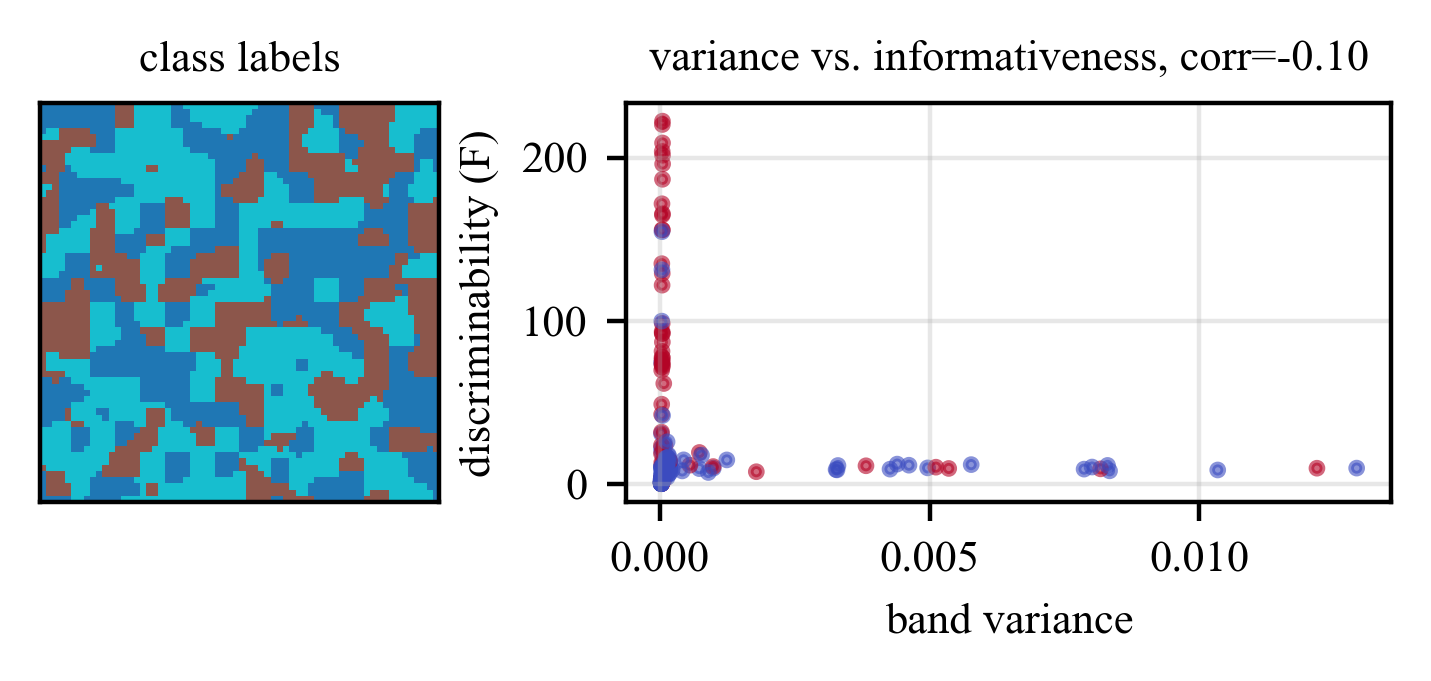
\includegraphics[width=\columnwidth]{fig_scene_v2.png}
\DIFaddendFL \caption{Variance is decoupled from informativeness. \DIFdelbeginFL \DIFdelFL{Each }\DIFdelendFL \DIFaddbeginFL \DIFaddFL{Left: class labels. Right: each }\DIFaddendFL point is a band \DIFaddbeginFL \DIFaddFL{(red}\DIFaddendFL : \DIFdelbeginFL \DIFdelFL{per-band
variance against per-band discriminability. The }\DIFdelendFL \DIFaddbeginFL \DIFaddFL{discriminative; blue: nuisance and scatter); the }\DIFaddendFL high-variance bands are nuisance \DIFdelbeginFL \DIFdelFL{and
}\DIFdelendFL \DIFaddbeginFL \DIFaddFL{or }\DIFaddendFL scatter\DIFdelbeginFL \DIFdelFL{bands}\DIFdelendFL , not \DIFdelbeginFL \DIFdelFL{the }\DIFdelendFL discriminative \DIFdelbeginFL \DIFdelFL{ones }\DIFdelendFL (correlation near zero), so \DIFdelbeginFL \DIFdelFL{ranking bands by
}\DIFdelendFL variance \DIFaddbeginFL \DIFaddFL{ranking }\DIFaddendFL fails.}
\label{fig:scene}
\end{figure}

\subsection{Artifacts, nonlinear physics, and clutter}\DIFaddbegin \label{sec:artifacts}
\DIFaddend On top of the clean cube the generator adds Rayleigh scatter at
$\lambda_\mathrm{em}=\lambda_\mathrm{ex}$ (with a second-order ghost at
$2\lambda_\mathrm{ex}$) and a water Raman line at a fixed wavenumber offset
($\approx 3400\,\mathrm{cm}^{-1}$), each scaled by a per-pixel turbidity field, then
Poisson shot noise and Gaussian read noise. Three optional effects introduce
concentration nonlinearity: a primary inner filter \DIFdelbegin \DIFdel{$\exp(-s A_\mathrm{ex})$}\DIFdelend \DIFaddbegin \DIFadd{$\exp(-s_\mathrm{ie} A_\mathrm{ex})$}\DIFaddend ;
\emph{reabsorption} \DIFdelbegin \DIFdel{$\exp(-s A_\mathrm{em}(\lambda))$}\DIFdelend \DIFaddbegin \DIFadd{$\exp(-s_\mathrm{re} A_\mathrm{em}(\lambda))$}\DIFaddend , whose overlap with the blue edge
of emission reshapes the band and relocates discriminative information into band shape;
and FRET, where a saturating fraction $E=k c_A/(1+k c_A)$ of donor energy is transferred
to a co-localized acceptor, encoding dye co-localization in a band ratio. Compactly,
the \DIFdelbegin \DIFdel{inner filter and transfer are
}\begin{displaymath}
\DIFdel{F = F_{\mathrm{obs}}\,10^{-(A_{\mathrm{ex}}+A_{\mathrm{em}})/2},
\qquad E=\frac{k\,c_A}{1+k\,c_A},
}\end{displaymath}%DIFAUXCMD
\DIFdelend \DIFaddbegin \DIFadd{attenuated signal and the transfer efficiency are
}\begin{equation}
\DIFadd{F_{\mathrm{obs}} = F\,e^{-s_{\mathrm{ie}}A_{\mathrm{ex}}}\,e^{-s_{\mathrm{re}}A_{\mathrm{em}}(\lambda_{\mathrm{em}})},
\qquad E=\frac{k\,c_A}{1+k\,c_A},
}\end{equation}\DIFaddend 
with \DIFdelbegin \DIFdel{reabsorption $A_{\mathrm{em}}(\lambda)=\sum_k \varepsilon_k c_k\,\alpha_k(\lambda)$ }\DIFdelend \DIFaddbegin \DIFadd{$A_{\mathrm{ex}}=\sum_k \varepsilon_k c_k a_k(\lambda_{\mathrm{ex}})$, dimensionless strength knobs
$s_{\mathrm{ie}},s_{\mathrm{re}}$ (not physical path lengths), reabsorption $A_{\mathrm{em}}(\lambda)=\sum_k \varepsilon_k c_k\,a_k(\lambda)$ (the excitation profile serves as absorption profile at the emission wavelength), }\DIFaddend and a
Raman line at $1/\lambda_R=1/\lambda_{\mathrm{ex}}-\Delta\bar\nu$. Finally,
fixed-pattern clutter injects many class-irrelevant low-rank spatial fields on random
band subsets, the analogue of illumination and detector artifacts and the dominant
real-instrument confound. By dialing these knobs \DIFdelbegin \DIFdel{the generator }\DIFdelend \DIFaddbegin \DIFadd{it }\DIFaddend spans \emph{clean}
(variance $\approx$ informativeness, an idealized baseline \DIFdelbegin \DIFdel{that }\DIFdelend real acquisitions never
meet), \emph{realistic}, \emph{clutter}, \emph{nonlinear} (reabsorption or FRET), and
\emph{spatial-texture} regimes \DIFdelbegin \DIFdel{from a single }\DIFdelend \DIFaddbegin \DIFadd{in one }\DIFaddend call.

\subsection{Ground truth, reproducibility, and real fluorophores}
Every render returns a ground-truth sidecar with concentration maps, clean cubes, and
per-fluorophore emission peaks, which enables a tight \emph{peak-recovery} metric (did a selected
band land within a tolerance of a true emission peak; a random selector scores about $0.33$) in
addition to \DIFdelbegin \DIFdel{broad }\DIFdelend information-retention metrics. The \DIFdelbegin \DIFdel{generator
exposes a one-call }\DIFdelend \DIFaddbegin \DIFadd{study scripts (}\DIFaddend \texttt{build\_dataset} \DIFdelbegin \DIFdel{API }\DIFdelend \DIFaddbegin \DIFadd{in }\texttt{\DIFadd{reports/}}\DIFadd{, not library API) call }\texttt{\DIFadd{render}} \DIFaddend with explicit knobs \DIFdelbegin \DIFdel{for size, emission
sampling, nuisance brightness, scatter, noise, clutter, and nonlinear physics; a script
re-runs every simulation and records exact parameters, so figures and numbers are
reproducible}\DIFdelend \DIFaddbegin \DIFadd{and record exact parameters}\DIFaddend . Parametric dyes can be replaced by \DIFdelbegin \DIFdel{real measured spectra
imported from FPbase, and an interactive workbench}\DIFdelend \DIFaddbegin \DIFadd{measured spectra
from a downloaded FPbase payload via a library importer (not yet exposed in the workbench). The in-development 3D workbench, SpectralForge Studio (Fig.~\ref{fig:gui}), }\DIFaddend lets a user \DIFdelbegin \DIFdel{paint concentration maps, render, and validate a selection }\DIFdelend \DIFaddbegin \DIFadd{place a lamp, camera, and samples in a 3D scene, render the 4D cube, and inspect it }\DIFaddend against ground truth.
\DIFdelbegin \DIFdel{This makes SpectralForge usable both as a controlled benchmark and as adesign tool for real 4D fluorescence experiments. As an
interactive application (}\DIFdelend \DIFaddbegin 

\begin{figure*}[p]
\centering
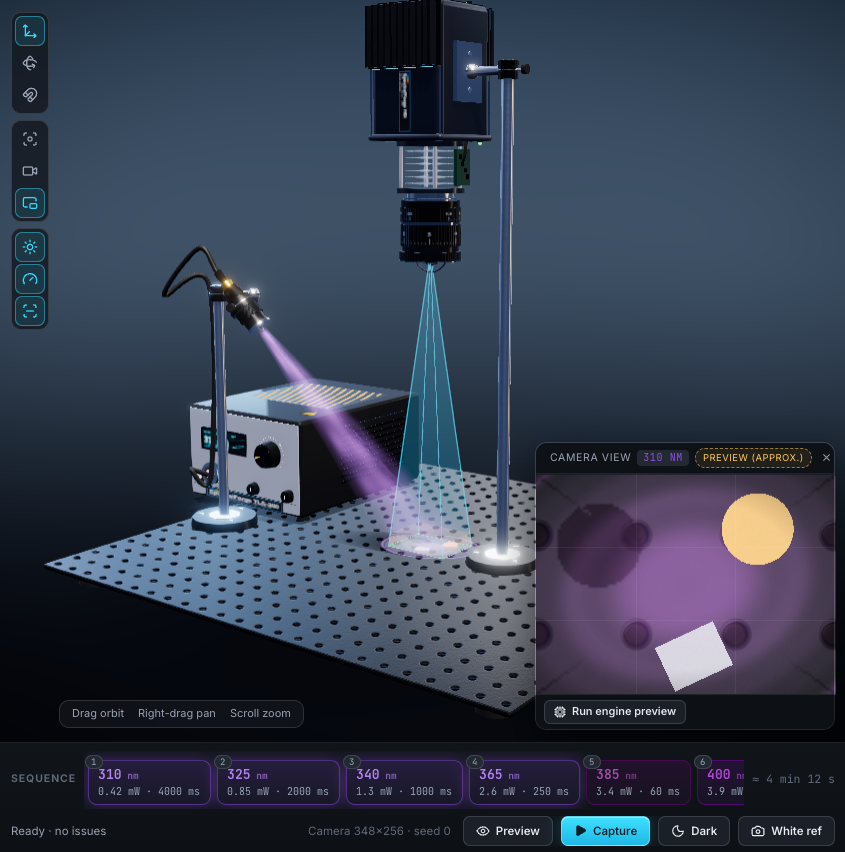
\includegraphics[width=0.405\textwidth]{fig_studio_design_crop.png}\hfill
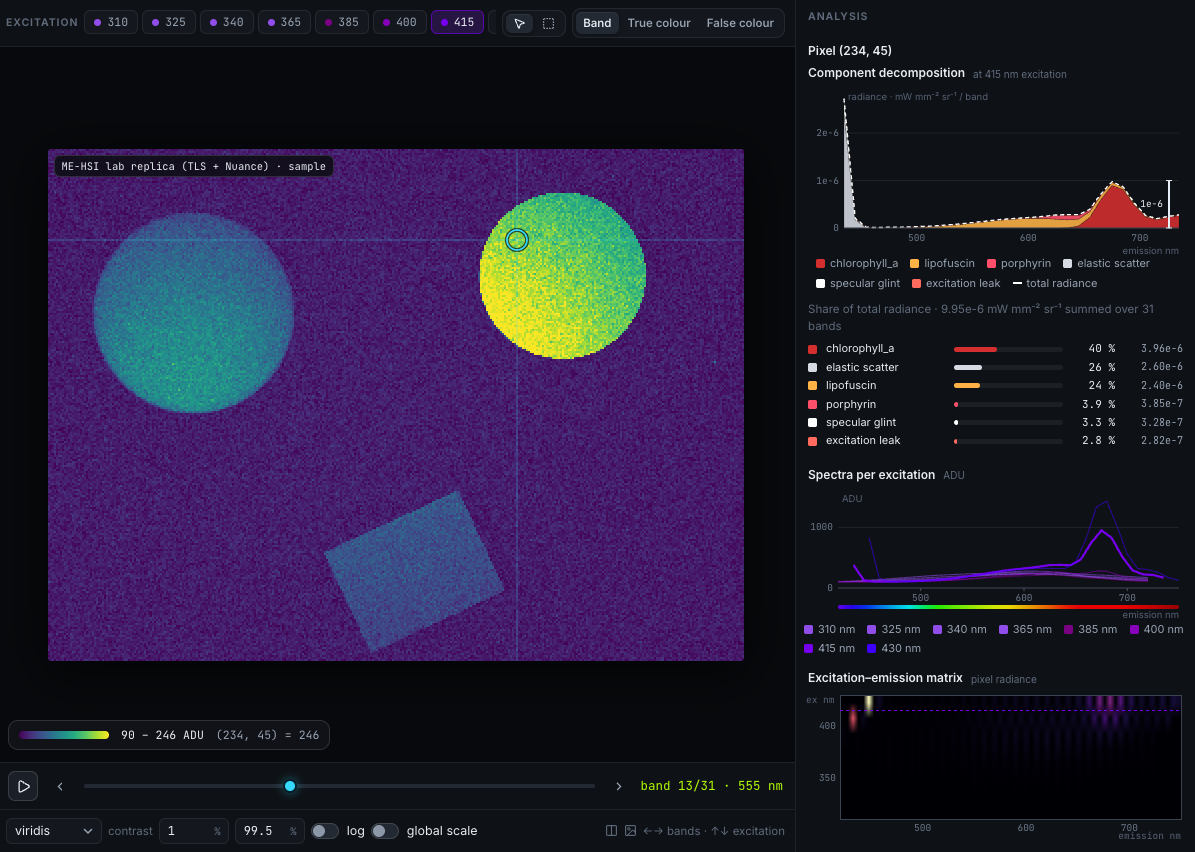
\includegraphics[width=0.575\textwidth]{fig_studio_explore_crop.png}
\caption{\DIFaddFL{SpectralForge Studio (in development). (a) Design: lamp, LCTF camera and samples placed in 3D, with the camera view. (b) Explore: a band image and, for the selected pixel, its ground-truth physical components, spectra and EEM. The study below used the core generator of Sec.~2, not Studio's added physics.}}
\label{fig:gui}
\end{figure*}

\begin{figure*}[p]
\centering
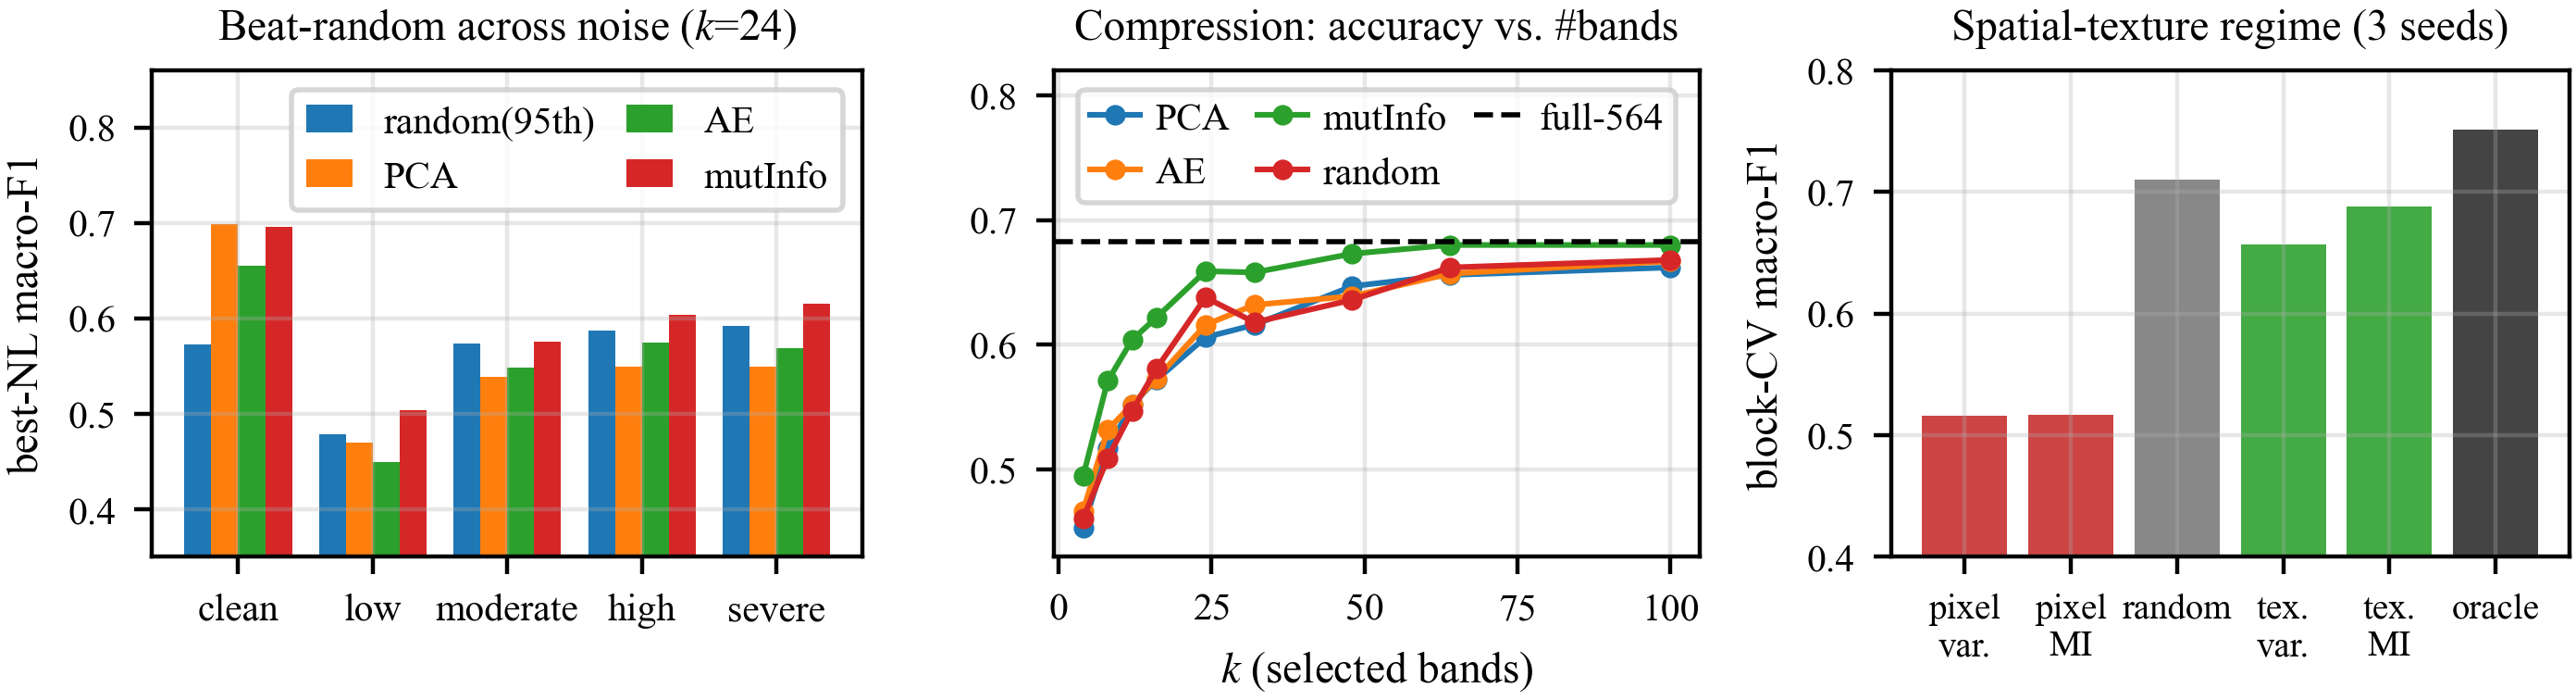
\includegraphics[width=\textwidth]{fig_results_v2.png}
\caption{\DIFaddFL{The benchmark in use. Left: beat-random across five noise levels at $k=24$ of 564 bands (Sec.~\ref{sec:grid}): blind PCA and autoencoder beat the random $95$th percentile only on clean data; under clutter only supervised MI does. Middle: compression over 4 to 100 bands; the autoencoder tracks PCA (about $95\%$ of the full spectrum); labels compress about $2.7\times$ better. Right: spatial texture (block CV): per-pixel selectors fall below random and no learned spatial selector beats it.}}
\label{fig:results}
\end{figure*}

\begin{figure*}[p]
\centering
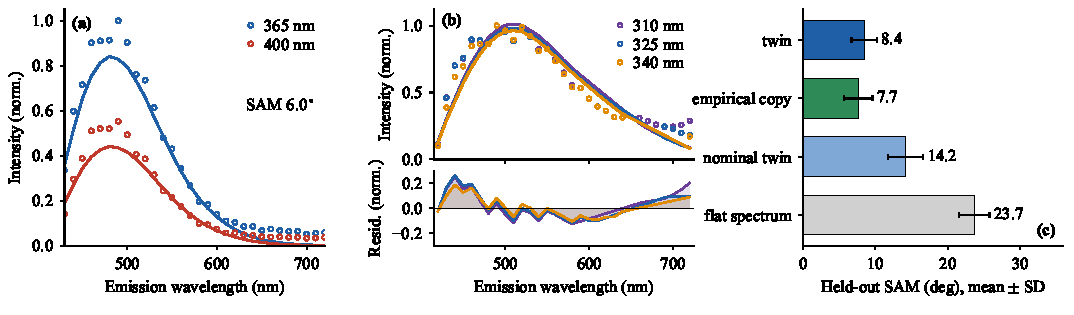
\includegraphics[width=\textwidth]{fig_realdata}
\caption{\DIFaddFL{Real-data validation. (a)~Drop 5 (median SAM): measured (markers) and predicted (lines) at held-out excitations. (b)~Collagen ROI 4 (median case of 24): measured, predicted and residual at held-out 310/325/340\,nm. (c)~Collagen held-out SAM, mean $\pm$ SD (24 cases).}}
\label{fig:realdata}
\end{figure*}

\subsection{\DIFadd{Validation against real acquisitions}}\label{sec:real}
\DIFadd{Fitting Eq.~(1), through a model of our tunable-lamp/LCTF instrument~\mbox{%DIFAUXCMD
\cite{ref_chil4d}}\hskip0pt%DIFAUXCMD
, to 4 excitations (310/340/385/415\,nm) of 16 fluorescent drops predicts the 3 held-out excitations without gain refit (median $R^2=0.96$, SAM $6.0^\circ$, Fig.~\ref{fig:realdata}a). For collagen, whose intensities are incomparable across excitations, only shape is testable: after per-excitation gain and smooth throughput correction, held-out SAM is $8.4\pm1.8^\circ$ and shape $R^2=0.83\pm0.13$ (24 cases; }\DIFaddend Fig.~\DIFdelbegin \DIFdel{\ref{fig:gui}), a user picks or defines fluorophores in a library (}\DIFdelend \DIFaddbegin \DIFadd{\ref{fig:realdata}b,c), slightly worse than copying another sample's spectrum ($7.7^\circ$).
}


\section{\DIFadd{Evaluation Protocol}}
\DIFadd{Two questions are kept apart: simulator fidelity, covered by the linearity tests of Sec.~2.2 and the real-data check of Sec.~\ref{sec:real}; and benchmark validity, covered by known ground truth plus random and full-spectrum controls, which need no claim that a simulated cube equals a real one. Table~\ref{tab:setup} summarizes the setup.
}

\begin{table}[t]
\caption{\DIFaddFL{Experimental setup and the reason for each element.}}
\label{tab:setup}
\centering
\small
\renewcommand{\arraystretch}{1.05}
\begin{tabular}{@{}p{0.15\linewidth}p{0.48\linewidth}p{0.27\linewidth}@{}}
\toprule
\DIFaddFL{Element }& \DIFaddFL{Setting }& \DIFaddFL{Why }\\
\midrule
\DIFaddFL{Selectors }& \DIFaddFL{variance; PCA loadings; AE (label-free); mutual information (labels) }& \DIFaddFL{naive to supervised }\\
\DIFaddFL{Regimes }& \DIFaddFL{clean; realistic; clutter; reabsorption; FRET; spatial texture }& \DIFaddFL{ideal to nonlinear }\\
\DIFaddFL{Noise }& \DIFaddFL{5 levels: photon scale $5\!\times\!10^4$ to $200$, Rayleigh $0.1$ to $0.7$, clutter $0$ to $4.5$ }& \DIFaddFL{gain under degradation }\\
\DIFaddFL{Classifiers }& \DIFaddFL{k-NN, RF, MLP, LR; macro-F1; CV (block CV for texture) }& \DIFaddFL{scored by downstream use }\\
\DIFaddFL{Controls }& \DIFaddFL{random subsets (95th pct.); full spectrum }& \DIFaddFL{chance; ceiling }\\
\DIFaddFL{Seeds }& \DIFaddFL{6 (Table~\ref{tab:battery}); 2 (}\DIFaddendFL Fig.~\DIFdelbeginFL \DIFdelFL{\ref{fig:gui_library}: excitation and emission peaks and widths, quantum
yield, extinction) , mixes them into materials that are concentration recipes, paints those
materials onto a canvas as layers, then acquires, renders the 4D cube, selects bands, and
validates against ground truth, all in one window}\DIFdelendFL \DIFaddbeginFL \DIFaddFL{\ref{fig:results}); 3 (texture) }& \DIFaddFL{paired CIs }\\
\DIFaddFL{Scene, grid }& \DIFaddFL{$64{\times}64$ px (Table~\ref{tab:battery}: $40{\times}40$), 3 classes; 564 or 228 bands (Sec.~\ref{sec:grid}) }& \DIFaddFL{known labels, peaks }\\
\bottomrule
\end{tabular}
\end{table}

\subsection{\DIFadd{Spectral grid}}\label{sec:grid}
\DIFadd{The study uses 4 excitations (405, 470, 488, 506\,nm) and emission from 420 to 700\,nm: every 2\,nm for Fig.~\ref{fig:results} ($141$ bands, $4\times141=564$ excitation-emission bands, the ``full-564'' classifier) and every 5\,nm for Table~\ref{tab:battery} ($57$ bands, $228$ features)}\DIFaddend .

\DIFdelbegin %DIFDELCMD < \begin{figure}[t]
%DIFDELCMD < \centering
%DIFDELCMD < 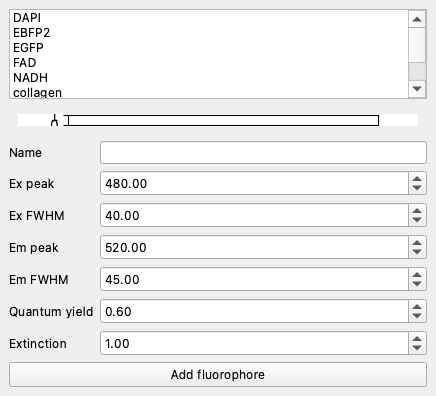
\includegraphics[width=0.80\linewidth]{fig_gui_library.png}
%DIFDELCMD < %%%
%DIFDELCMD < \caption{%
{%DIFAUXCMD
\DIFdelFL{Defining a fluorophore in the workbench library: choose a built-in dye or enter
excitation and emission peaks and widths, quantum yield, and extinction. Materials are
concentration mixtures of these fluorophores.}}
%DIFAUXCMD
%DIFDELCMD < \label{fig:gui_library}
%DIFDELCMD < \end{figure}
%DIFDELCMD < 

%DIFDELCMD < \begin{figure*}[!tb]
%DIFDELCMD < \centering
%DIFDELCMD < 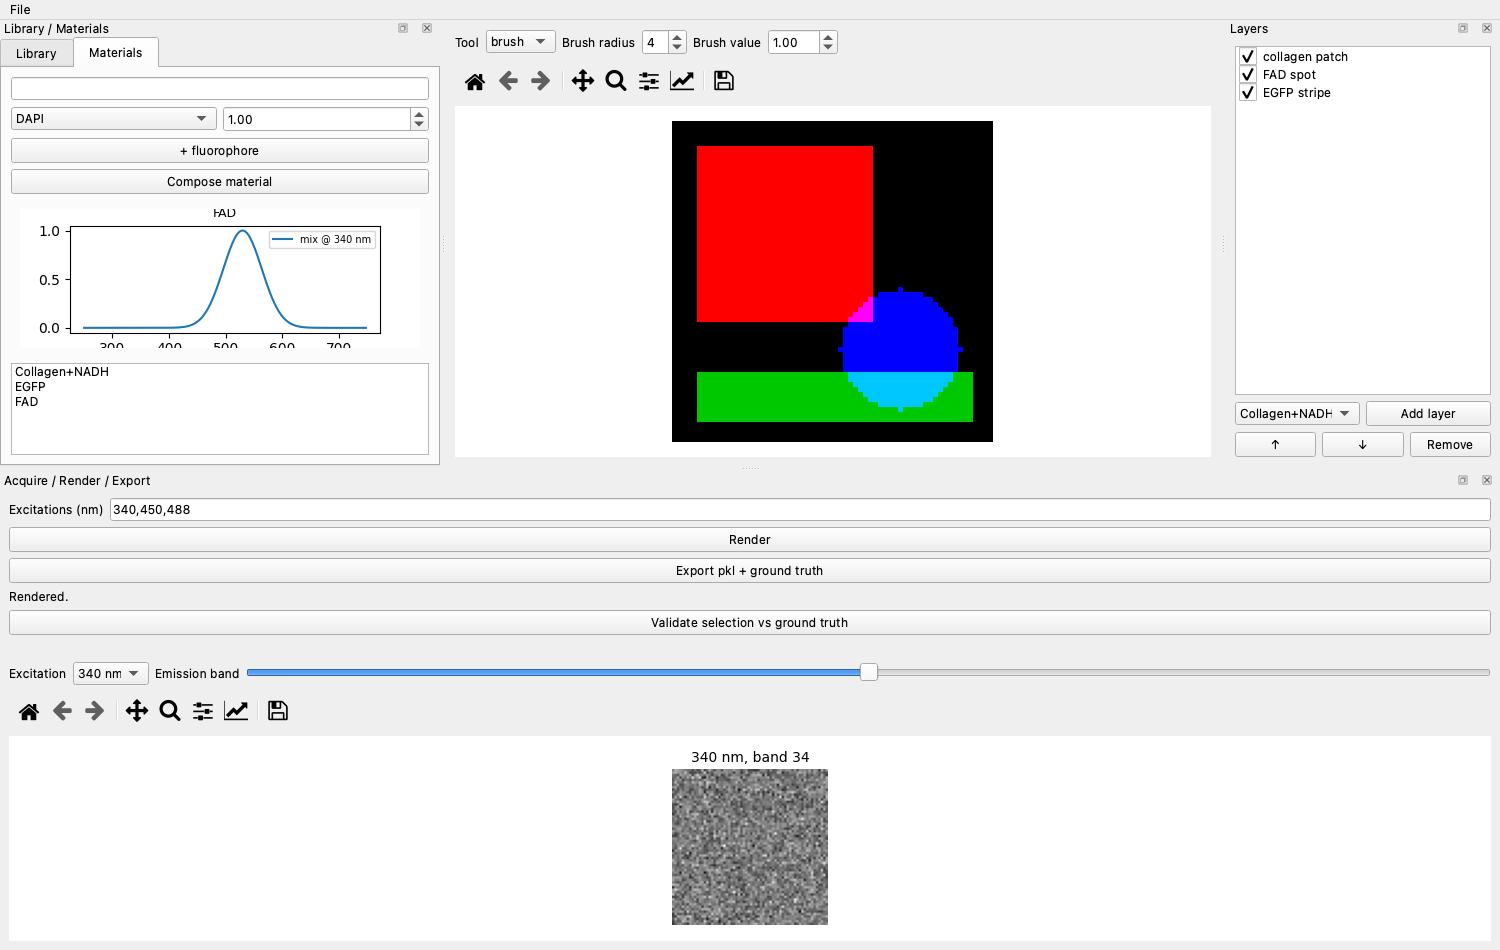
\includegraphics[width=0.84\textwidth]{fig_gui.png}
%DIFDELCMD < %%%
%DIFDELCMD < \caption{%
{%DIFAUXCMD
\DIFdelFL{The SpectralForge workbench. Left: fluorophore recipes (materials) with a live spectrum.
Centre: the painted canvas (a collagen and NADH patch, an FAD spot, an EGFP stripe), coloured by
class label. Right: the layer stack. Bottom: acquire, render, and one-click validation against
ground truth, here previewing a rendered emission band at 340\,nm.}}
%DIFAUXCMD
%DIFDELCMD < \label{fig:gui}
%DIFDELCMD < \end{figure*}
%DIFDELCMD < 

%DIFDELCMD < %%%
\section{\DIFdel{Evaluation Protocol}}
%DIFAUXCMD
\addtocounter{section}{-1}%DIFAUXCMD
\DIFdelend Selection quality is the accuracy of a downstream classifier \DIFdelbegin \DIFdel{trained }\DIFdelend on the selected bands, \DIFdelbegin \DIFdel{using labels
}\DIFdelend \DIFaddbegin \DIFadd{with labels
used }\DIFaddend only at evaluation time. We score each subset with a classifier
panel (k-nearest neighbors, random forest, MLP, logistic regression), cross-validated,
reporting macro-F1 and, on nonlinear regimes, a \emph{nonlinear-only gap} (the accuracy
an expressive model recovers beyond a linear one), because a linear metric cannot credit
a nonlinear-shape selection. Two controls matter here. A \textbf{random}
baseline: a method that cannot beat the $95$th percentile of random band subsets adds
nothing. And the \textbf{full spectrum}: the accuracy ceiling a selector tries to
approach. Where
discrimination is spatial we use spatial-block cross-validation to remove
spatial-autocorrelation leakage.
\DIFdelbegin \DIFdel{These two controls, often absent in prior work, guard
against reporting a gain that a random subset would already reach.
}\DIFdelend 

\section{Using the Benchmark}
Band selection, which removes non-informative bands to shrink a real hyperspectral
acquisition~\DIFdelbegin \DIFdel{\mbox{%DIFAUXCMD
\cite{ref_guan,ref_scirep}}\hskip0pt%DIFAUXCMD
}\DIFdelend \DIFaddbegin \DIFadd{\mbox{%DIFAUXCMD
\cite{ref_guan,ref_scirep,ref_bsnet} }\hskip0pt%DIFAUXCMD
(its collagen and lichen data are public~\mbox{%DIFAUXCMD
\cite{ref_zen_collagen,ref_zen_lichens}}\hskip0pt%DIFAUXCMD
)}\DIFaddend , is one thing SpectralForge is built to test, so we exercise it with a
panel of standard selectors: variance ranking, PCA loadings\DIFaddbegin \DIFadd{~\mbox{%DIFAUXCMD
\cite{ref_jolliffe}}\hskip0pt%DIFAUXCMD
}\DIFaddend , supervised mutual information (a
labels-using reference), and a fully unsupervised \DIFdelbegin \DIFdel{autoencoder-with-latent-perturbation
}\DIFdelend \DIFaddbegin \DIFadd{autoencoder~\mbox{%DIFAUXCMD
\cite{ref_hinton}}\hskip0pt%DIFAUXCMD
-with-latent-perturbation
}\DIFaddend selector, which reconstructs the standardized cube, perturbs each latent dimension, and
turns the per-band reconstruction sensitivity into a per-band influence. The \DIFdelbegin \DIFdel{generator
supplies the cubes and their ground truth; the protocol above scores each subset. The
question is not which selector wins but whether the benchmark behaves as designed, that
is, whether }\DIFdelend \DIFaddbegin \DIFadd{question is whether }\DIFaddend decoupling variance from informativeness makes \DIFdelbegin \DIFdel{it }\DIFdelend \DIFaddbegin \DIFadd{the benchmark }\DIFaddend discriminate methods and regimes.

It does. On confounded scenes a variance ranker \DIFdelbegin \DIFdel{barely beats random }\DIFdelend \DIFaddbegin \DIFadd{does no better than, and usually below, random subsets (e.g.\ $0.40$ vs $0.45$ on the realistic regime)}\DIFaddend . PCA loadings is the
strongest blind selector only in the idealized \emph{clean} regime, where the informative
bands are also the brightest. No real fluorescence acquisition reaches that regime, since
real cubes always carry scatter, autofluorescence, and noise; once those enter, on the
realistic and FRET regimes, the two selectors tie. Label-free selection \DIFaddbegin \DIFadd{marginally }\DIFaddend overtakes PCA only
where the physics places discriminative information in nonlinear band \emph{shape}, as under
reabsorption (macro-F1 $0.449$ vs $0.431$, \DIFaddbegin \DIFadd{bootstrap }\DIFaddend $95\%$ CI $[+0.001,+0.029]$, Cohen
$d\approx+0.94$\DIFdelbegin \DIFdel{; its }\DIFdelend \DIFaddbegin \DIFadd{, but paired Wilcoxon $p=0.16$, so the gain is marginal; the AE-MLP }\DIFaddend subset carries nonlinear-only
information \DIFdelbegin \DIFdel{$+0.030$ that the linear
selector's does not, $-0.021$}\DIFdelend \DIFaddbegin \DIFadd{$+0.014$, the conv-AE $-0.001$, against $-0.016$ for PCA loadings}\DIFaddend ; Table~\ref{tab:battery}). The pattern is a general one:
\emph{informative implies has variance implies PCA-selectable}, so a nonlinear
\emph{classification} task need not imply a nonlinear \emph{selection} task, and the
benchmark separates the two.
\DIFdelbegin \DIFdel{This regime map, not a single winner, is what the benchmark
reports.
}\DIFdelend 

\begin{table}[t]
\caption{Label-free \DIFdelbeginFL \DIFdelFL{autoencoder }\DIFdelendFL \DIFaddbeginFL \DIFaddFL{AE }\DIFaddendFL vs.\ the strongest blind baseline (PCA loadings): best-of-panel macro-F1\DIFdelbeginFL \DIFdelFL{over }\DIFdelendFL \DIFaddbeginFL \DIFaddFL{, }\DIFaddendFL six seeds\DIFdelbeginFL \DIFdelFL{. Bold marks the }\DIFdelendFL \DIFaddbeginFL \DIFaddFL{; bold is }\DIFaddendFL better\DIFdelbeginFL \DIFdelFL{selector}\DIFdelendFL \DIFaddbeginFL \DIFaddFL{. Clean margin: paired Wilcoxon $p=0.03$}\DIFaddendFL ; \DIFdelbeginFL \DIFdelFL{the clean and
}\DIFdelendFL reabsorption\DIFdelbeginFL \DIFdelFL{margins are significant at }\DIFdelendFL \DIFaddbeginFL \DIFaddFL{: bootstrap }\DIFaddendFL $95\%$ \DIFdelbeginFL \DIFdelFL{, the }\DIFdelendFL \DIFaddbeginFL \DIFaddFL{CI excludes zero but $p=0.16$ (marginal); }\DIFaddendFL rest are ties.}
\label{tab:battery}
\centering
\DIFdelbeginFL %DIFDELCMD < \footnotesize
%DIFDELCMD < \setlength{\tabcolsep}{4.5pt}
%DIFDELCMD < \renewcommand{\arraystretch}{1.15}
%DIFDELCMD < \begin{tabular}{@{}lccl@{}}
%DIFDELCMD < %%%
\DIFdelendFL \DIFaddbeginFL \renewcommand{\arraystretch}{1.2}
\begin{tabular*}{\columnwidth}{@{\extracolsep{\fill}}lccl@{}}
\DIFaddendFL \toprule
Regime & AE & PCA-load & verdict \\
\midrule
clean & 0.590 & \textbf{0.635} & linear suffices \\
realistic & 0.527 & 0.531 & tie \\
reabsorption & \textbf{0.449} & 0.431 & \DIFdelbeginFL \DIFdelFL{label-free wins }\DIFdelendFL \DIFaddbeginFL \DIFaddFL{marginal AE gain }\DIFaddendFL \\
FRET & 0.635 & 0.642 & tie \\
\bottomrule
\DIFdelbeginFL %DIFDELCMD < \end{tabular}
%DIFDELCMD < %%%
\DIFdelendFL \DIFaddbeginFL \end{tabular*}
\DIFaddendFL \end{table}


\DIFdelbegin %DIFDELCMD < \begin{figure*}[!tb]
%DIFDELCMD < \centering
%DIFDELCMD < 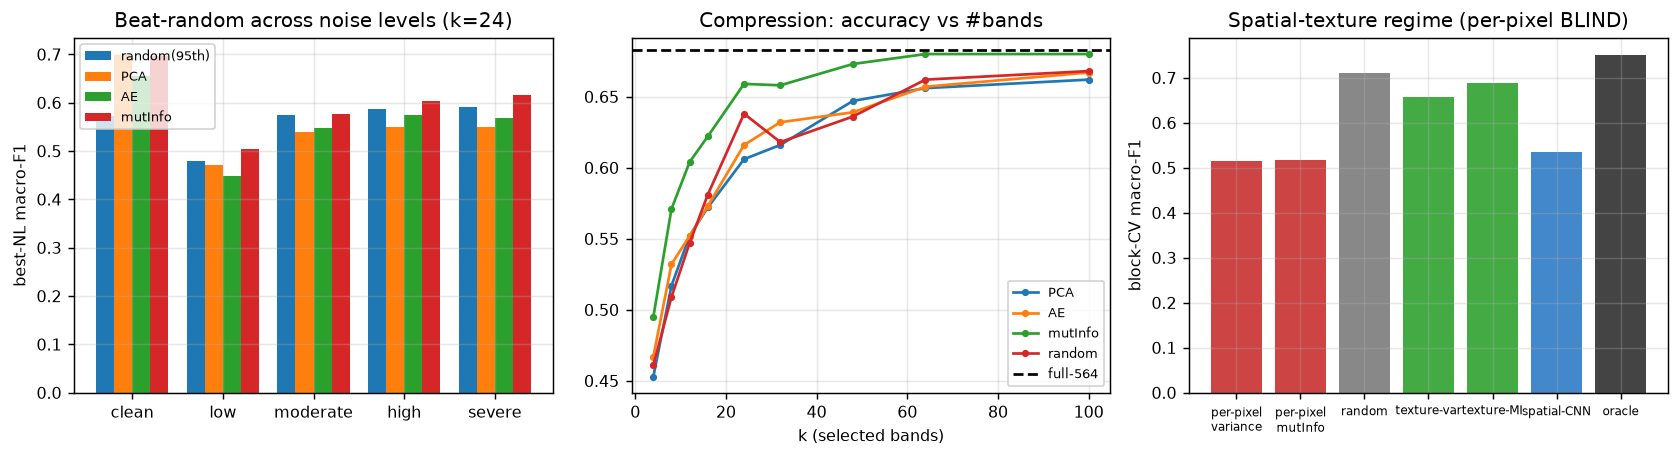
\includegraphics[width=0.98\textwidth]{fig_results.png}
%DIFDELCMD < %%%
%DIFDELCMD < \caption{%
{%DIFAUXCMD
\DIFdelFL{The benchmark in use. Left: beat-random across five noise levels: blind
PCA and autoencoder selection beat the random $95$th percentile only on clean data, and
under clutter only supervised mutual information does. Middle: compression curve: the
autoencoder tracks PCA at every budget, both reaching about $95\%$ of the full spectrum,
while labels compress about $2.7\times$ better. Right: the spatial-texture regime under
block cross-validation: per-pixel selectors are the worst (below random) because
the classes have identical per-pixel spectra, and only a spatial model with the right
bands reaches the oracle.}}
%DIFAUXCMD
%DIFDELCMD < \label{fig:results}
%DIFDELCMD < \end{figure*}
%DIFDELCMD < 

%DIFDELCMD < %%%
\DIFdelend The random and full-spectrum controls also mark the limits (Fig.~\ref{fig:results}).
Under fixed-pattern clutter no blind selector beats a random subset, because clutter is
high-variance but class-irrelevant; there only label-aware selection helps. No selector
beats the full spectrum, so selection buys compression, not accuracy, and blind subsets
are unstable band to band (Jaccard about $0.1$ to $0.2$), which favors selecting spectral
regions or consensus sets. And when class is carried by spatial texture, so that every
class shares the same per-pixel spectrum, per-pixel selection falls below random (\DIFaddbegin \DIFadd{three seeds, }\DIFaddend $0.52$ \DIFdelbegin \DIFdel{to
$0.55$, }\DIFdelend against a random \DIFdelbegin \DIFdel{$0.674$)while a spatial model with the right bands reaches the
oracle ($0.78$). These are properties the benchmark makes visible, and they answer the practical questions: when to select bands, when to keep the spectrum, and when
the problem is spatial rather than spectral}\DIFdelend \DIFaddbegin \DIFadd{$0.71$), the oracle bands reach $0.75$, and none of the spatial selectors we tried
(texture variance or MI, $0.66$ to $0.69$; a spatial CNN, $0.53$ in a separate finer configuration with random $0.58$) beats random, so spatial selection remains open}\DIFaddend .

\section{Discussion and Conclusion}
SpectralForge gives 4D fluorescence imaging an open, physically realistic source of cubes
with perfect ground truth, so \DIFdelbegin \DIFdel{that }\DIFdelend methods can be \DIFdelbegin \DIFdel{designed, tested , and compared
}\DIFdelend \DIFaddbegin \DIFadd{tested }\DIFaddend before scarce instrument time is spent.
\DIFdelbegin \DIFdel{The band-selection study is one demonstration of
that value. Paired with a protocol whose }\DIFdelend \DIFaddbegin \DIFadd{With }\DIFaddend random and full-spectrum controls\DIFdelbegin \DIFdel{check that a
reported gain is real}\DIFdelend , the simulator turns ``does this selector help'' into a measured, reproducible question, and its answer is specific: PCA loadings is the strongest blind
baseline only in the idealized clean regime that no real acquisition reaches, ties
label-free selection once realistic scatter and noise enter, and is \DIFdelbegin \DIFdel{overtaken only }\DIFdelend \DIFaddbegin \DIFadd{only marginally overtaken }\DIFaddend where
the physics is nonlinear.

While SpectralForge captures key primary photophysical phenomena, the simulator operates
under certain physical and optical simplifications. Currently, inner-filter attenuation and
reabsorption are modeled using first-order exponential path approximations rather than full
3D radiative transfer or Monte Carlo photon transport through dense scattering media.
Furthermore, the instrument model assumes an idealized optical train with spatially uniform
illumination, uniform spectral detector response, and static photophysics, omitting dynamic
exposure photobleaching kinetics during sequence acquisition as well as chromatic
aberrations and thermal drift. Expanding the engine to incorporate full radiative transport
and dynamic bleaching models remains an important direction for future extensions\DIFdelbegin \DIFdel{.
}\DIFdelend \DIFaddbegin \DIFadd{; the in-development workbench (Fig.~\ref{fig:gui}) already adds 3D Monte Carlo transport and photobleaching.
}\DIFaddend 

\DIFdelbegin \DIFdel{The same generator supports experiment planning, algorithm prototyping, and teaching.
}\DIFdelend A natural next step is to evaluate performance on complex, multi-component target samples
(heterogeneous biological tissues, environmental specimens, or engineered multi-fluorophore
composites), where informative spectral structure is decoupled from overall band variance.
SpectralForge and its workbench are in active development toward a production release, and
the authors can provide exclusive early access to interested laboratories and individuals
on request (\DIFdelbegin \DIFdel{please }\DIFdelend contact the corresponding author by email); the full experiment record
\DIFdelbegin \DIFdel{accompanying }\DIFdelend \DIFaddbegin \DIFadd{for }\DIFaddend this study is released for reproducible use.

\section*{Acknowledgment}
\DIFaddbegin {\setlength{\emergencystretch}{2em}\DIFaddend Financial support from the European Union NAS SAR-101087403 \DIFdelbegin \DIFdel{and the United States
R44 HL120511 awards }\DIFdelend \DIFaddbegin \DIFadd{award }\DIFaddend is gratefully acknowledged. A large-language-model assistant was
used for code scaffolding, figure generation, and language editing; the design,
analysis, and conclusions are the authors' own and were verified by them.\DIFaddbegin \par}
\DIFaddend 

\begin{thebibliography}{00}
\bibitem{ref_lakowicz} J. R. Lakowicz, \emph{Principles of Fluorescence Spectroscopy},
3rd ed. Springer, 2006.
\bibitem{ref_kasha} M. Kasha, ``Characterization of electronic transitions in complex
molecules,'' \emph{Discuss. Faraday Soc.}, vol.~9, pp.~14--19, 1950.
\bibitem{ref_valeur} B. Valeur and M. N. Berberan-Santos, \emph{Molecular Fluorescence},
2nd ed. Wiley-VCH, 2012.
\bibitem{ref_bro} R. Bro, ``PARAFAC: Tutorial and applications,'' \emph{Chemom. Intell. Lab. Syst.}, vol.~38, pp.~149--171, 1997.
\bibitem{ref_jablonski} A. Jab\l{}o\'nski, ``Efficiency of anti-Stokes fluorescence in
dyes,'' \emph{Nature}, vol.~131, pp.~839--840, 1933.
\bibitem{ref_hinton} G. E. Hinton and R. R. Salakhutdinov, ``Reducing the dimensionality
of data with neural networks,'' \emph{Science}, vol.~313, pp.~504--507, 2006.
\bibitem{ref_jolliffe} I. T. Jolliffe, \emph{Principal Component Analysis}, 2nd ed.
Springer, 2002.
\bibitem{ref_bsnet} Y. Cai, X. Liu, and Z. Cai, ``BS-Nets: An end-to-end framework for
band selection of hyperspectral image,'' \emph{IEEE \DIFdelbegin \DIFdel{Trans. Geosci. Remote Sens.}\DIFdelend \DIFaddbegin \DIFadd{TGRS}\DIFaddend },
vol.~58, no.~3, pp.~1969--1984, 2020.
\bibitem{ref_mercader} M. Mercader, L. Swift, S. Sood, H. Asfour, M. Kay, and
N. Sarvazyan, ``Use of endogenous NADH fluorescence for real-time in situ visualization
of epicardial radiofrequency ablation lesions and gaps,'' \emph{Am. J. Physiol. Heart Circ.\DIFdelbegin \DIFdel{Physiol.}\DIFdelend }, vol.~302, no.~10, pp.~H2131--H2138, 2012.
\bibitem{ref_gil} D. A. Gil, L. M. Swift, H. Asfour, N. Muselimyan, M. A. Mercader, and
N. A. Sarvazyan, ``Autofluorescence hyperspectral imaging of radiofrequency ablation
lesions in porcine cardiac tissue,'' \emph{J. Biophotonics}, vol.~10, no.~8,
pp.~1008--1017, 2017.
\bibitem{ref_guan} S. Guan, H. Asfour, N. Sarvazyan, and M. Loew, ``Application of
unsupervised learning to hyperspectral imaging of cardiac ablation lesions,'' \emph{J.
Med. Imaging}, vol.~5, no.~4, art.~046003, 2018.
\bibitem{ref_chil4d} N. Chilingaryan, F. Villarruel, T. Soghomonyan, V. Yeghiazaryan, and
N. Sarvazyan, ``4D hyperspectral imaging for intraoperative tissue classification,'' in
\emph{\DIFdelbegin \DIFdel{Medical }\DIFdelend \DIFaddbegin \DIFadd{Proc. SPIE Med. }\DIFaddend Imaging\DIFdelbegin \DIFdel{2025: Clinical and Biomedical Imaging}\DIFdelend }, vol.~\DIFdelbegin \DIFdel{13410. SPIE}\DIFdelend \DIFaddbegin \DIFadd{13410}\DIFaddend , 2025, pp.~255--260.
\bibitem{ref_chillichen} N. Chilingaryan, A. Gasparyan, and N. Sarvazyan, ``Multi-excitation
hyperspectral imaging toward improved lichen identification,'' in \emph{Proc. \DIFdelbegin \DIFdel{15th Workshop
on Hyperspectral Imaging and Signal Processing: Evol. in Remote Sensing (}\DIFdelend WHISPERS\DIFdelbegin \DIFdel{)}\DIFdelend }\DIFdelbegin \DIFdel{. IEEE}\DIFdelend , 2025, pp.~1--5.
\bibitem{ref_hunanyan} A. Hunanyan, N. Ter-Petrosyan, F. Villarruel, T. Soghomonyan,
N. Sarvazyan, A. Butavyan, and V. Yeghiazaryan, ``Deep learning classification of ablated
atrial tissue in multi-excitation hyperspectral images,'' in \emph{Proc. \DIFdelbegin \DIFdel{15th Workshop on
Hyperspectral Imaging and Signal Processing: Evol. in Remote Sensing (}\DIFdelend WHISPERS\DIFdelbegin \DIFdel{)}\DIFdelend }\DIFdelbegin \DIFdel{. IEEE}\DIFdelend , 2025, pp.~1--5.
\bibitem{ref_scirep} N. Meloyan and N. Sarvazyan, ``Unsupervised deep learning for
wavelength selection in multi-excitation fluorescence imaging,'' \emph{Scientific Reports}
\DIFdelbegin \DIFdel{(minor revision), 2025.
}\DIFdelend \DIFaddbegin \DIFadd{under review, 2026.
}\bibitem{ref_zen_collagen} \DIFadd{K. Ghahramanyan, ``250929\_Collagen,'' dataset, Zenodo, 2026, doi: 10.5281/zenodo.20677504.
}\bibitem{ref_zen_lichens} \raggedright \DIFadd{N. Chilingaryan and N. Sarvazyan, ``250707\_}\allowbreak \DIFadd{4DHSI\_}\allowbreak \DIFadd{Lichens\_}\allowbreak \DIFadd{Palette,'' dataset, Zenodo, 2026, doi:~10.5281/}\allowbreak \DIFadd{zenodo.18640119.
}\DIFaddend \end{thebibliography}

\end{document}
